\documentclass[11pt,a4paper]{article}

\usepackage[spanish]{babel}
\usepackage{amsmath}
\usepackage{amssymb}
\usepackage{graphicx}
\usepackage{booktabs}
\usepackage[numbers]{natbib}
\usepackage{geometry}
\usepackage[hidelinks]{hyperref}

\graphicspath{{results/figures/}{../results/figures/}}

\geometry{margin=2.5cm}

\title{Optimización de redes neuronales con algoritmos genéticos (neuroevolución)}
\author{Nombre de los autores}
\date{}

\begin{document}

\maketitle

\section{Resumen}

Este proyecto desarrolla desde cero algoritmos genéticos para optimizar redes neuronales en dos vertientes, comparándolos siempre con líneas base en igualdad de presupuesto. En la primera, se evolucionan directamente los pesos de una red neuronal de control en CartPole-v1, entorno cuya función de recompensa no admite gradientes útiles. El algoritmo (selección por torneo y ruleta, elitismo, cruces de un punto, uniforme y BLX-$\alpha$, mutación gaussiana y mixta) resuelve la tarea en 5 de 5 semillas con 470 evaluaciones de media, frente a 700 de la búsqueda aleatoria y 3933 episodios de REINFORCE, que solo alcanza el objetivo en 3 de 5 ejecuciones. La comparación de operadores sitúa la ruleta (220 evaluaciones) y BLX-$\alpha$ (310) por delante del cruce de un punto (470) y del uniforme (550). En la segunda vertiente, el algoritmo actúa como optimizador de caja negra de la arquitectura y los hiperparámetros de una red entrenada con descenso por gradiente sobre el conjunto tabular UCI Letter Recognition, con un cromosoma mixto de 10 genes: alcanza 0,9619 de exactitud en validación frente a 0,9501 de la búsqueda aleatoria y 0,8733 de la configuración por defecto, con 0,9612 en test. La evaluación paralela de poblaciones, verificada con semillas preasignadas, logra una aceleración de 4,76$\times$ en 12 núcleos. Los resultados concluyen que la evolución es más eficiente y fiable que la suerte y que el gradiente en este tipo de tareas, con las salvedades estadísticas de 5 semillas y de un solo problema por vertiente documentadas en la discusión.

\section{Introducción y motivación}

El aprendizaje automático moderno se apoya casi por completo en el descenso por gradiente: para entrenar una red neuronal basta con escribir una pérdida diferenciable y propagar sus derivadas hacia atrás. Sin embargo, hay problemas prácticos donde ese camino se corta. En tareas de control, como mantener un polo en equilibrio sobre un carrito, la calidad de un controlador se mide por un resultado simulado (pasos de supervivencia) que no admite derivadas útiles respecto a los pesos. En el diseño de redes, además, la \emph{estructura} misma (número de capas, anchos, tasa de aprendizaje, regularización) es una decisión \emph{discreta} y mixta sobre la que el gradiente no define una dirección.

Los algoritmos evolutivos ofrecen una respuesta unificada a ambos huecos: solo necesitan \emph{medir} cuán bueno es un candidato, nunca diferenciarlo. Este proyecto, propuesta A4 de la asignatura \emph{Optimización y Heurística}, desarrolla desde cero un algoritmo genético y lo aplica en dos vertientes complementarias:

\begin{enumerate}
  \item \textbf{Pesos en CartPole}: evolucionar directamente los pesos de una red neuronal de control en el entorno \emph{CartPole-v1} de Gymnasium \citep{brockman2016}, donde la función objetivo no es diferenciable, y comparar el resultado con una búsqueda aleatoria y con REINFORCE \citep{williams1992}, el método de gradiente canónico para políticas.
  \item \textbf{Arquitectura e hiperparámetros en UCI}: usar el AG como optimizador de caja negra de la configuración de una red mayor entrenada con descenso por gradiente (PyTorch) sobre el conjunto tabular \emph{Letter Recognition} \citep{frey1991}, comparándolo con búsqueda aleatoria y con una configuración por defecto.
\end{enumerate}

La motivación es doble. Desde el punto de vista científico, las dos vertientes ilustran cuándo compite la evolución con el gradiente: cuando el objetivo es no diferenciable (vertiente 1) y cuando el espacio de decisión es mixto y evaluable solo mediante un procedimiento de entrenamiento completo (vertiente 2). Desde el punto de vista práctico, obliga a enfrentarse a los problemas reales de cualquier metaheurística: igualdad de presupuestos con las líneas base, varianza propia de los métodos estocásticos (múltiples semillas, medias y desviaciones), coste computacional de la evaluación (paralelización y medición del \emph{speedup}) y reproducibilidad estricta (semillas fijas y scripts que regeneran figuras y tablas).

El resto de la memoria se organiza así: se revisa el estado del arte (sección~\ref{sec:estado}), se formula matemáticamente ambos problemas (sección~\ref{sec:formulacion}), se describen los métodos (sección~\ref{sec:metodos}), su implementación (sección~\ref{sec:implementacion}) y los datos (sección~\ref{sec:datos}); después se presentan los experimentos y resultados (sección~\ref{sec:experimentacion}), se discuten con sus limitaciones (sección~\ref{sec:discusion}) y se concluyen (sección~\ref{sec:conclusiones}).

\section{Descripción del problema y estado del arte}

Pendiente: revisión de la literatura con referencias reales (algoritmos genéticos, estrategias evolutivas, NEAT, CMA-ES, métodos de gradiente para control y búsqueda de hiperparámetros).

\section{Formulación matemática}

Pendiente: variables de decisión (cromosoma de pesos en CartPole; cromosoma mixto de arquitectura e hiperparámetros en UCI), función objetivo (recompensa media; accuracy de validación), tipo de problema y restricciones (rangos de genes, presupuesto de evaluaciones).

\section{Métodos}

\subsection{Algoritmo genético general}

Ambas vertientes comparten un único motor evolutivo, implementado desde cero y desacoplado del dominio: recibe una función de \emph{fitness}, un inicializador y los operadores genéticos como parámetros. Su esqueleto es el clásico ciclo de generaciones con evaluación por presupuesto:

\begin{enumerate}
  \item \textbf{Inicializar}: muestrear $P$ candidatos aleatorios.
  \item \textbf{Evaluar}: puntuar toda la población (aquí radica el cuello de botella computacional).
  \item \textbf{Registrar}: mejor, media y desviación de la generación, y evaluaciones acumuladas.
  \item \textbf{Elitismo}: copiar intactos los $e$ mejores a la siguiente generación.
  \item \textbf{Seleccionar}: elegir progenitores con torneo ($k=3$) o ruleta.
  \item \textbf{Recombinar y mutar}: generar los $P-e$ hijos restantes.
  \item Repetir hasta agotar el presupuesto $N$ de evaluaciones (enteras: $N/P$ generaciones).
\end{enumerate}

El mejor-so-far nunca decrece gracias al elitismo, y el presupuesto \emph{exacto} de evaluaciones garantiza comparaciones justas frente a las líneas base.

\subsection{Selección}

\paragraph{Torneo con $k=3$.}
Para cada hueco de progenitor se extraen $k$ índices uniformemente sin reemplazo y se devuelve el de mayor fitness:
\begin{equation}
  i^* = \arg\max_{i \in S_k} F(x_i), \qquad S_k \sim \text{Uniforme}(\{1,\dots,P\}, k).
\end{equation}
La presión de selección crece con $k$: con $k=1$ todos tienen igual probabilidad y con $k=P$ siempre gana el mejor (estancamiento). $k=3$ equilibra explotación y diversidad.

\paragraph{Ruleta (proporcional al fitness).}
Probabilidad $p_i = f_i / \sum_j f_j$ con los fitness desplazados a positivos, $f_i = F(x_i) - \min_j F(x_j) + \varepsilon$, $\varepsilon = 10^{-12}$, porque la fórmula exige valores estrictamente positivos. Cuando un individuo domina claramente, su porción de ruleta aplasta a los demás y la diversidad colapsa: es la debilidad clásica de este operador, que en nuestros experimentos se matiza porque el fitness es ruidoso (cada evaluación usa condiciones iniciales distintas) y el elitismo protege al mejor sin depender de la selección.

\subsection{Operadores de cruce}

\paragraph{Un punto.}
Se corta el cromosoma en un punto aleatorio $c \in \{1,\dots,n-1\}$ y se intercambian las colas: los bloques contiguos (una capa completa de la red) se preservan íntegros.

\paragraph{Uniforme.}
Gen a gen, cada hijo toma el valor de uno de los progenitores con probabilidad $1/2$:
\begin{equation}
  h_j = \begin{cases} a_j & \text{con prob. } 1/2 \\ b_j & \text{con prob. } 1/2 \end{cases}
  \qquad j = 1,\dots,n.
\end{equation}
Mezcla máxima, ideal cuando los genes son independientes: es el cruce empleado en el cromosoma de 10 hiperparámetros, donde cada gen codifica una decisión distinta.

\paragraph{BLX-$\alpha$.}
Para pesos reales, cada gen hijo se muestrea uniformemente del intervalo que une a los progenitores ampliado un factor $\alpha = 0{,}5$ a ambos lados, con $d_j = |a_j - b_j|$:
\begin{equation}
  h_j \sim \mathcal{U}\!\left( \min(a_j, b_j) - \alpha d_j,\ \max(a_j, b_j) + \alpha d_j \right).
\end{equation}
Hereda lo bueno de ambos y explora \emph{fuera} de ellos sin saltos descontrolados. En la comparación de operadores de CartPole, BLX-$\alpha$ alcanzó la puntuación perfecta antes que los otros dos cruces.

\subsection{Mutación}

\paragraph{Gaussiana para pesos.}
Cada gen se muta con probabilidad $\rho = 0{,}1$ añadiendo ruido $\mathcal{N}(0, \sigma^2)$ con $\sigma = 0{,}1$: afinamiento local alrededor de lo que la selección ya construyó.

\paragraph{Mixta para hiperparámetros.}
Con probabilidad $\rho = 0{,}3$ por gen, el ruido se adapta al \emph{tipo} del gen: los índices discretos (capas, anchos, lote) se redondean y recortan a su rango entero; el gen de activación \emph{cicla} a otra activación distinta; los continuos (dropout, tasas en escala logarítmica) reciben ruido gaussiano $\sigma = 0{,}3$. Todo se recorta a la caja $\mathcal{X}$ permitida.

\subsection{Línea base: búsqueda aleatoria}

Mismo presupuesto de evaluaciones y mismo inicializador que el AG, sin selección ni recombinación: se muestrean candidatos i.i.d. y se conserva el mejor. Es la referencia que responde ``¿aporta algo la evolución frente a la suerte?''.

\subsection{Línea base de gradiente: REINFORCE}

Entrenamos una política estocástica con la red NumPy de la Fase 1, con $\pi_w(a \mid s) = \text{softmax}(f_w(s))$, muestreando acciones. Tras cada episodio se actualiza en sentido ascenso de gradiente con la regla
\begin{equation}
  w \leftarrow w + \frac{\nu}{B} \sum_{e=1}^{B} \sum_{t} \big( G_t^{(e)} - \bar{b}^{(e)} \big)\, \nabla_w \log \pi_w\!\left( a_t^{(e)} \mid s_t^{(e)} \right),
\end{equation}
donde $G_t$ es el retorno desde el paso $t$ (recompensa unitaria, sin descuento), $\bar{b}$ la media de retornos del lote de $B = 10$ episodios (línea base que reduce la varianza sin sesgar el estimador) y $\nu = 0{,}001$ la tasa de aprendizaje. La identidad $\nabla_z \log \pi(a \mid s) = \mathbb{1}[a] - \text{softmax}(z)$ en las salidas permite propagar el error hacia atrás a mano (la verificamos por diferencias finitas en los tests). Con $\nu = 0{,}01$ la política \emph{colapsó} (media final $\approx 9{,}4$ pasos): la suma de gradientes a lo largo de hasta 500 pasos amplifica cada actualización y destruye la estructura aprendida; la tasa 10 veces menor converge de forma estable. Este contraste (el AG nunca usa gradientes; REINFORCE se construye solo con ellos) es el eje de la comparación.

\subsection{Paralelización}

La evaluación de una población se reparte entre procesos con \texttt{ProcessPoolExecutor}: cada tarea lleva su cromosoma y una semilla de evaluación \emph{preasignada} (dibujada antes del despacho), de modo que el resultado no depende del orden de programación de los procesos. Los trabajadores cargan el dataset una sola vez (inicializador del pool), se descartan tareas de más de un gen (\texttt{chunksize=1}) para equilibrar la carga cuando los tiempos de episodio varían $\times 50$, y se realiza una ejecución de calentamiento sin cronometrar para no medir el arranque de procesos. La ganancia se mide como $S(p) = t_{\text{secuencial}} / t_p$ frente a la línea ideal $S(p) = p$ (ver sección~\ref{sec:experimentacion}).

\section{Implementación}

\subsection{Organización del código}

El repositorio separa por responsabilidades el dominio, la evolución y los experimentos:

\begin{itemize}
  \item \texttt{src/networks/}: \texttt{numpy\_mlp.py} (red completa en NumPy: aplanado, reconstrucción de matrices y paso hacia adelante) y \texttt{torch\_mlp.py} (configuración \texttt{MLPConfig}, construcción y bucle de entrenamiento con PyTorch).
  \item \texttt{src/genetic/}: \texttt{engine.py} (motor evolutivo), \texttt{selection.py}, \texttt{operators.py} (cruces y mutación gaussiana), \texttt{mixed\_operators.py} y \texttt{hyperparams\_chromosome.py} (codificación mixta de hiperparámetros), \texttt{random\_search.py}.
  \item \texttt{src/environments/} y \texttt{src/evaluation/}: evaluadores de CartPole y de configuraciones UCI, ambos con evaluación paralela y semillas preasignadas.
  \item \texttt{src/baselines/}: \texttt{reinforce.py} (línea base de gradiente en NumPy puro, con retropropagación manual).
  \item \texttt{src/uci/}, \texttt{data/}: descarga, parsing y preprocesado del dataset.
  \item \texttt{src/utils/}: métricas compartidas, gráficas en español y utilidades de semillas.
  \item \texttt{tests/} (seis baterías), \texttt{experiments/} (cinco scripts reproducibles), \texttt{results/} (figuras y logs).
\end{itemize}

\subsection{Decisiones de diseño}

\begin{enumerate}
  \item \textbf{Motor desacoplado del dominio (SRP/OCP).} \texttt{run\_genetic\_algorithm} no importa ni CartPole ni PyTorch: recibe \texttt{fitness\_fn} (o un evaluador por lote \texttt{population\_fitness\_fn}), el inicializador y los operadores como llamables inyectados. El mismo motor ejecutó la función esfera en los tests, CartPole y la búsqueda de hiperparámetros sin una sola línea de cambio.
  \item \textbf{Funciones puras y semillas explícitas.} Los operadores nunca mutan sus entradas y todos los módulos de azar reciben un \texttt{rng} explícito: cada resultado es reproducible a partir de su semilla y las pruebas pueden comparar ejecuciones completas.
  \item \textbf{Un único formato de resultado.} \texttt{EvolutionResult} (mejor, historia por generación y curvas ya expuestas como arrays) lo comparten el AG y la búsqueda aleatoria, lo que permite gráficas y métricas genéricas.
  \item \textbf{Evaluación paralela reproducible.} Las semillas de evaluación se sortean \emph{antes} de despachar las tareas y viajan dentro de cada tarea; así el orden en que el sistema operativo programe los procesos no afecta al resultado (verificado con tests que comparan 1, 2 y 3 trabajadores). El pool es persistente y se calienta una vez fuera de la medición; en UCI cada trabajador carga el dataset una sola vez mediante el inicializador del pool.
  \item \textbf{Codificación mixta tipada.} Tasas de aprendizaje y weight decay en escala logarítmica, anchos y lote como potencias de dos, activación como índice categórico con mutación cíclica, y recorte a la caja permitida en decodificación y mutación.
  \item \textbf{Determinismo completo.} Semillas en NumPy, en \texttt{torch.manual\_seed} y en el generador de barajado del \texttt{DataLoader}; \texttt{torch.set\_num\_threads(1)} evita contención de hilos entre trabajadores paralelos.
  \item \textbf{Verificación numérica del gradiente.} La retropropagación manual de REINFORCE se valida contra diferencias finitas del log-verosimilitud ponderado (tolerancia $10^{-4}$): un error de signo o de máscara ReLU saltaría inmediatamente en los tests.
\end{enumerate}

\subsection{Dificultades encontradas}

\begin{enumerate}
  \item \textbf{La búsqueda aleatoria saturaba CartPole.} Con la red pequeña de 58 pesos, los controladores aleatorios que estabilizaban el polo eran demasiado densos: la suerte competía con la evolución. Se corrigió el protocolo (fitness robusto con condiciones iniciales nuevas en cada evaluación) y se aumentó la red a $(4,16,16,2)$, donde la evolución sí aporta de forma medible.
  \item \textbf{El módulo de velocidad medía el arranque de procesos.} Las primeras mediciones daban speedup $0{,}17\times$: el cronómetro incluía el arranque de los trabajadores (segundos, por importar \texttt{gymnasium} en un sistema de ficheros lento). Se añadió una calentamiento explícito con un flujo de semillas separado.
  \item \textbf{REINFORCE colapsó con tasa $0{,}01$.} La actualización suma gradientes de hasta 500 pasos y destruyó la política (media final $\approx 9{,}4$). La sonda con $0{,}001$ y $0{,}0001$ mostró que solo $10^{-3}$ aprende de forma estable; se cambió el valor por defecto con la evidencia medida.
  \item \textbf{Perturbar la solución la destruía.} Para construir la población ``evolucionada'' del benchmark se añadió ruido $\sigma = 0{,}01$ al mejor cromosoma y la media se desplomó de 500 a 59: un controlador resuelto vive en el filo del caja (cambios mínimos en los pesos invierten decisiones de empuje). Se usaron réplicas exactas.
  \item \textbf{Ruido de fin de línea en Git.} Windows/VS Code reescribía los ficheros con CRLF y ensuciaba cada diff; se añadió \texttt{.gitattributes} con \texttt{eol=lf}.
  \item \textbf{Incompatibilidad de versiones.} Los \texttt{pines} de \texttt{requirements.txt} (p.\ ej.\ \texttt{numpy==2.2.6}) no tienen ruedas para Python 3.14; se documentó la versión soportada y se ejecutó el desarrollo con numpy 2.5.4 sin observar diferencias funcionales.
\end{enumerate}

\section{Datos}

Pendiente: origen, DOI y licencia del dataset Letter Recognition, descripción de los 16 atributos y 26 clases, preprocesado (partición oficial, estandarización ajustada solo sobre entrenamiento) y particiones utilizadas.

\section{Experimentación y resultados}
\label{sec:experimentacion}

\subsection{Diseño experimental común}

Todos los experimentos comparten un protocolo de rigor: (i) \emph{igualdad de presupuesto} entre métodos comparados; (ii) múltiples semillas de ejecución (5 en todos los casos) con media, desviación típica muestral (división por $n-1$) y curvas de convergencia con banda de una desviación; (iii) fitness robusto en CartPole: cada evaluación usa condiciones iniciales nuevas, sorteadas con semillas preasignadas; (iv) separación estricta entrenamiento/validación/test en la vertiente UCI. Las figuras se regeneran íntegramente con los scripts de \texttt{experiments/} (verificado: los tres experimentos de NumPy reproducen bytes idénticos en cualquier máquina).

\subsection{Coste computacional: speedup de la evaluación paralela}

Se cronometra la misma tarea de evaluación de poblaciones de 50 redes $(4,16,16,2)$ con 5 repeticiones por configuración, en una máquina de 12 núcleos, con calentamiento previo de los procesos. Dos cargas de trabajo: \emph{ligera} (población aleatoria, episodios de $\approx$10 pasos) y \emph{pesada} (población evolucionada que sobrevive episodios completos, la situación real de las generaciones tardías).

\begin{table}[htbp]
  \centering
  \caption{Tiempo medio por población (s) y aceleración frente al secuencial.}
  \label{tab:speedup}
  \begin{tabular}{lcccccc}
    \toprule
    Procesos & 1 & 2 & 4 & 8 & 12 & \\
    \midrule
    Población aleatoria (s) & 0,251 & 0,156 & 0,096 & 0,079 & 0,086 & \multicolumn{1}{r}{(sec.: 0,226)} \\
    Aceleración & 0,90$\times$ & 1,45$\times$ & 2,36$\times$ & 2,85$\times$ & 2,63$\times$ & \\
    Población evolucionada (s) & 2,320 & 1,285 & 0,851 & 0,559 & 0,475 & \multicolumn{1}{r}{(sec.: 2,264)} \\
    Aceleración & 0,98$\times$ & 1,76$\times$ & 2,66$\times$ & 4,05$\times$ & \textbf{4,76$\times$} & \\
    \bottomrule
  \end{tabular}
\end{table}

\begin{figure}[htbp]
  \centering
  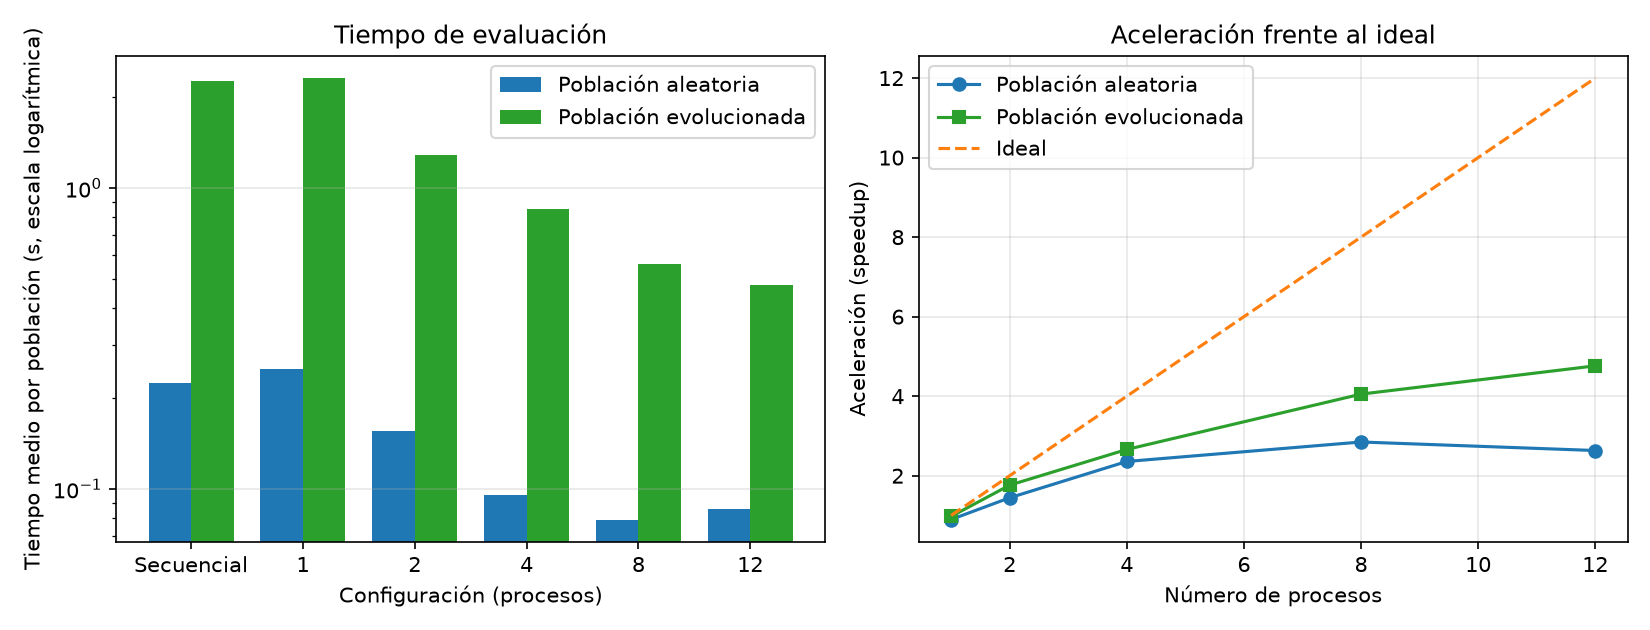
\includegraphics[width=0.95\linewidth]{parallel_speedup.png}
  \caption{Tiempo de evaluación (izquierda, escala logarítmica) y aceleración frente al ideal (derecha) para cargas ligera y pesada.}
  \label{fig:speedup}
\end{figure}

La carga pesada alcanza \textbf{4,76$\times$ con 12 procesos}, mientras la ligera se estanca en 2,85$\times$ y empeora a 12 (2,63$\times$): cuando cada tarea dura milisegundos, la coordinación entre procesos supera al trabajo ahorrado. Ninguna curva llega a la ideal $S(p)=p$ por (a) el coste de serializar cromosomas y recoger resultados y (b) la ley de Amdahl: la parte no paralelizable (creación de población, selección, cruce, mutación) limita el máximo. Con un trabajador el pool cuesta prácticamente nada (0,90--0,98$\times$), lo que confirma que la medición ya no incluye el arranque de procesos.

\subsection{CartPole: algoritmo genético frente a búsqueda aleatoria}

Con la red $(4,16,16,2)$, población 50, 3000 evaluaciones y 5 semillas (figura~\ref{fig:cartpole}):

\begin{table}[htbp]
  \centering
  \caption{Resultados en CartPole-v1 (5 semillas, 3000 evaluaciones).}
  \label{tab:cartpole}
  \begin{tabular}{lccc}
    \toprule
    Método & Mejor final (media $\pm$ dt) & Éxito (500) & Evaluaciones hasta 500 (media $\pm$ dt) \\
    \midrule
    Algoritmo genético & 500,0 $\pm$ 0,0 & 5/5 & 470 $\pm$ 317 \\
    Búsqueda aleatoria & 487,2 $\pm$ 28,6 & 4/5 & 700 $\pm$ 402 \\
    \bottomrule
  \end{tabular}
\end{table}

\begin{figure}[htbp]
  \centering
  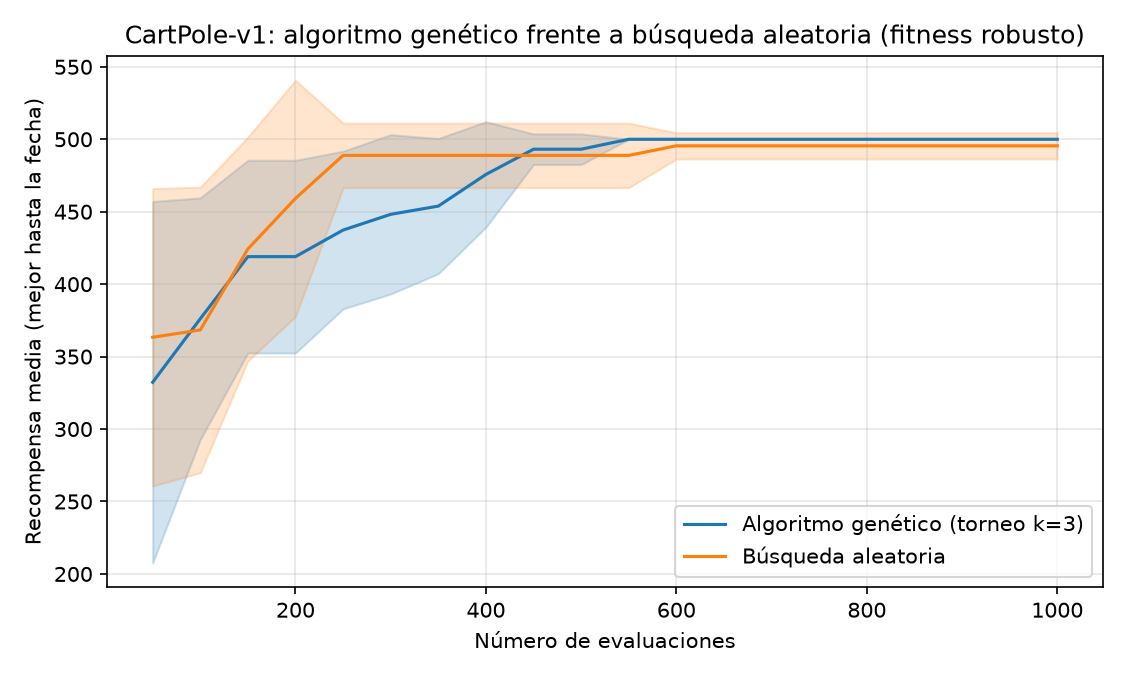
\includegraphics[width=0.85\linewidth]{phase1_ga_vs_random.png}
  \caption{CartPole-v1 (red 4-16-16-2): mejor hasta la fecha frente a evaluaciones, media de 5 semillas con banda de una desviación típica.}
  \label{fig:cartpole}
\end{figure}

El AG resuelve las 5 semillas y llega al óptimo $\approx$1,5$\times$ antes que la búsqueda aleatoria entre las ejecuciones exitosas. Dato preliminar relevante para la discusión: con la red \emph{pequeña} de 58 pesos, la búsqueda aleatoria saturaba el entorno (bastaba con suerte para estabilizar el polo), por lo que el protocolo se endureció con fitness robusto y una red mayor.

\subsection{Comparación de operadores genéticos}

Cuatro configuraciones (selección $\times$ cruce) con 5 semillas y 3000 evaluaciones cada una, todo lo demás idéntico:

\begin{table}[htbp]
  \centering
  \caption{Evaluaciones hasta la puntuación perfecta (media $\pm$ dt sobre las 5 semillas).}
  \label{tab:operadores}
  \begin{tabular}{lccc}
    \toprule
    Configuración & Éxito & Hasta 500 & Mejor final \\
    \midrule
    Ruleta + cruce un punto & 5/5 & \textbf{220 $\pm$ 220} & 500 $\pm$ 0 \\
    Torneo + BLX-$\alpha$ & 5/5 & 310 $\pm$ 290 & 500 $\pm$ 0 \\
    Torneo + cruce un punto & 5/5 & 470 $\pm$ 317 & 500 $\pm$ 0 \\
    Torneo + cruce uniforme & 5/5 & 550 $\pm$ 580 & 500 $\pm$ 0 \\
    \bottomrule
  \end{tabular}
\end{table}

\begin{figure}[htbp]
  \centering
  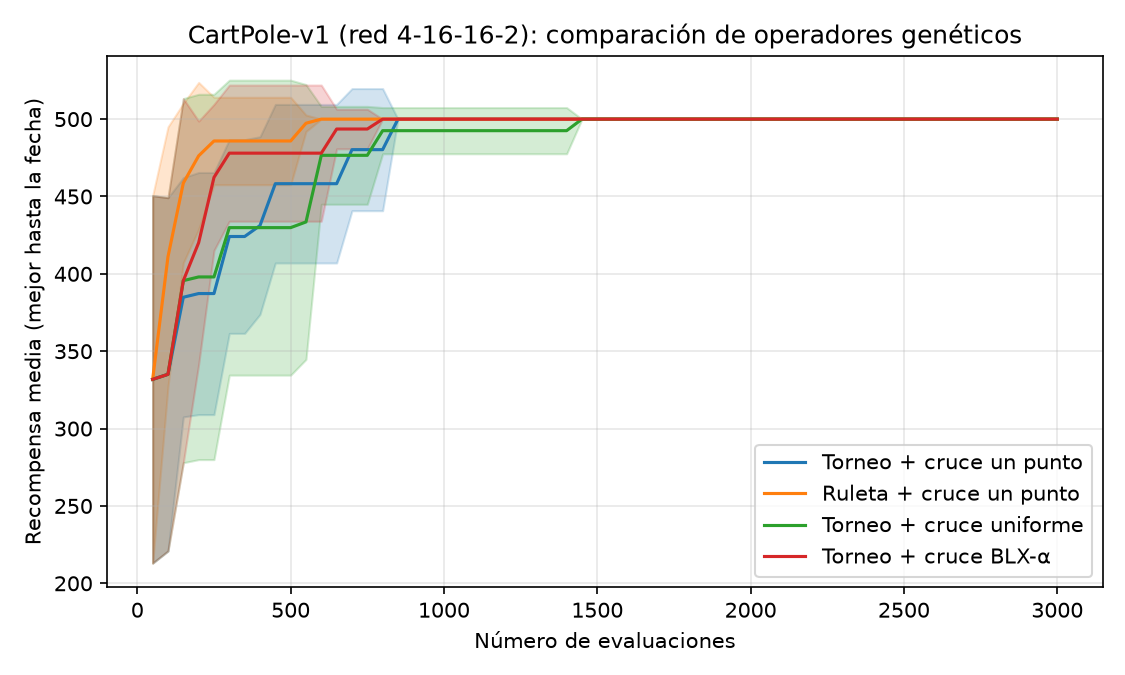
\includegraphics[width=0.85\linewidth]{operator_comparison.png}
  \caption{Comparación de operadores genéticos en CartPole-v1 (red 4-16-16-2).}
  \label{fig:operadores}
\end{figure}

Todas las configuraciones saturan la tarea, así que la discriminación está en la \emph{eficiencia}: la ruleta alcanza el óptimo antes que el torneo en \emph{todas} las semillas (4 victorias y 1 empate por parejas), seguida de BLX-$\alpha$, que confirma la ventaja teórica de muestrear en torno a los progenitores para pesos reales; el cruce uniforme, que destroza bloques de genes coadaptados, es el más lento y el más variable. La ausencia de estancamiento de la ruleta se explica porque el fitness es ruidoso (nadie puede monopolizar la selección) y el elitismo protege al mejor sin depender de la selección.

\subsection{Comparación a igual presupuesto de episodios: AG, aleatoria y REINFORCE}

Las tres compiten con el mismo presupuesto de 9000 episodios (el AG y la aleatoria lo consumen como 3000 evaluaciones $\times$ 3 episodios; REINFORCE entrena 9000 episodios), sobre un eje común de episodios jugados:

\begin{table}[htbp]
  \centering
  \caption{Comparación con igual presupuesto de 9000 episodios (5 semillas).}
  \label{tab:tresmetodos}
  \begin{tabular}{lccc}
    \toprule
    Método & Éxito (500) & Episodios hasta 500 & Mejor final \\
    \midrule
    Algoritmo genético & 5/5 & \textbf{1261 $\pm$ 952} & 500,0 $\pm$ 0,0 \\
    Búsqueda aleatoria & 5/5 & 2791 $\pm$ 2198 & 500,0 $\pm$ 0,0 \\
    REINFORCE ($\nu = 0{,}001$) & 3/5 & 3933 $\pm$ 1511 & 464,2 $\pm$ 70,9 \\
    \bottomrule
  \end{tabular}
\end{table}

\begin{figure}[htbp]
  \centering
  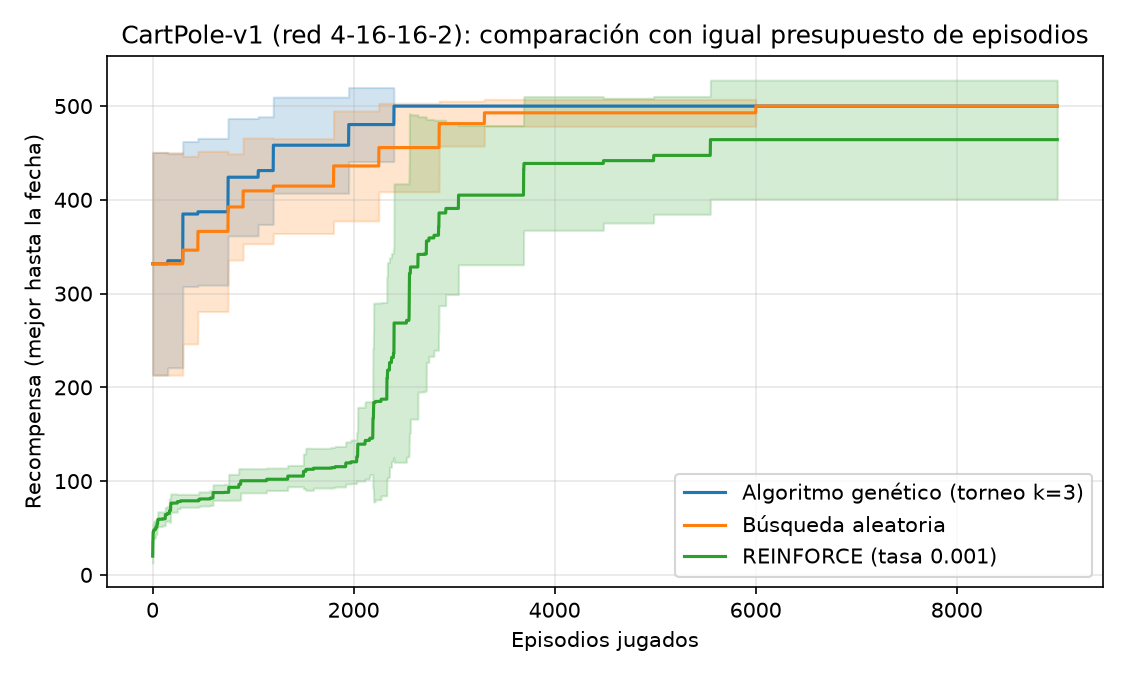
\includegraphics[width=0.85\linewidth]{reinforce_comparison.png}
  \caption{Comparación con igual presupuesto de episodios en CartPole-v1 (red 4-16-16-2).}
  \label{fig:tresmetodos}
\end{figure}

El AG alcanza el óptimo con \textbf{2,2}$\times$ menos episodios que la aleatoria y \textbf{3,1}$\times$ menos que REINFORCE, y es el único método fiable en todas las semillas. La curva de REINFORCE muestra su patrón clásico: meseta inicial $\approx$100 pasos durante 2000 episodios, despegue entre 2200 y 3500 y techo con banda muy ancha (alto sesgo de varianza del estimador de política). Con la tasa $0{,}01$ aprobada inicialmente la política \emph{colapsaba}; la sonda con $10^{-3}$ fue la más rápida que aprende de forma estable.

\subsection{Letter Recognition: arquitectura e hiperparámetros}

Presupuesto de 240 evaluaciones por semilla (población 20, 20 épocas de entrenamiento cada evaluación, 8 procesos), fitness en validación y evaluación final en test:

\begin{table}[htbp]
  \centering
  \caption{Exactitud (media $\pm$ dt, 5 semillas) en Letter Recognition.}
  \label{tab:letter}
  \begin{tabular}{lccc}
    \toprule
    Método & Validación & Test & Tiempo medio de búsqueda \\
    \midrule
    Algoritmo genético & \textbf{0,9619 $\pm$ 0,0044} & \textbf{0,9612 $\pm$ 0,0098} & 637,9 s \\
    Búsqueda aleatoria & 0,9501 $\pm$ 0,0079 & 0,9540 $\pm$ 0,0096 & 561,7 s \\
    Configuración por defecto (1 ejec.) & 0,8733 $\pm$ 0,0021 & 0,8856 $\pm$ 0,0036 & --- \\
    \bottomrule
  \end{tabular}
\end{table}

\begin{figure}[htbp]
  \centering
  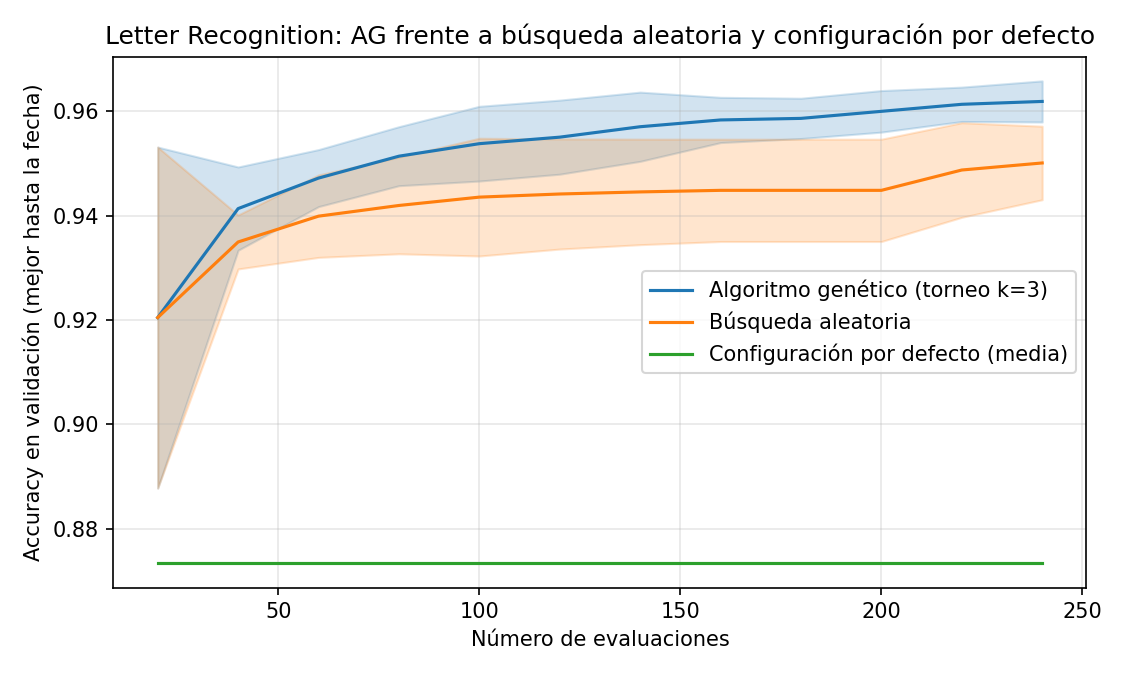
\includegraphics[width=0.85\linewidth]{phase3_ga_vs_random.png}
  \caption{Letter Recognition: AG frente a búsqueda aleatoria y a la configuración por defecto (media de validación).}
  \label{fig:letter}
\end{figure}

El AG supera a la búsqueda aleatoria en validación en \emph{todas} las semillas (5/5 por parejas) y ambos superan ampliamente a la configuración por defecto (8--9 puntos porcentuales). En test la ventaja del AG se reduce a 0,7--1,2 puntos con desviaciones de $\approx$1 punto: la comparación honesta es la de test (ver discusión). La re-ejecución íntegra en otra máquina reprodujo las conclusiones con diferencias de cuarto decimal, atribuibles a la no-exactitud de las rutinas BLAS de PyTorch entre hardware distinto (la versión canónica de la figuras~\ref{fig:letter} y su log es la del repositorio).

\section{Discusión}
\label{sec:discusion}

Pendiente: interpretación crítica de los resultados (por qué la búsqueda aleatoria satura CartPole con redes pequeñas, por qué la ruleta no se estancó, el papel del fitness ruidoso, el problema de varianza de REINFORCE, validez estadística con 5 semillas) y limitaciones del trabajo.

\section{Conclusiones y trabajo futuro}
\label{sec:conclusiones}

Pendiente: conclusiones de las dos vertientes del proyecto y trabajo futuro (NEAT, CMA-ES, más entornos, búsqueda bayesiana de hiperparámetros como referencia moderna).

\section*{Referencias}

\begin{thebibliography}{99}

\bibitem{goldberg1989}
D. E. Goldberg, \emph{Genetic Algorithms in Search, Optimization and Machine Learning}, Addison-Wesley, 1989.

\bibitem{holland1975}
J. H. Holland, \emph{Adaptation in Natural and Artificial Systems}, University of Michigan Press, 1975.

\bibitem{rechenberg1973}
I. Rechenberg, \emph{Evolutionsstrategie: Optimierung technischer Systeme nach Prinzipien der biologischen Evolution}, Frommann-Holzboog, 1973.

\bibitem{schwefel1995}
H.-P. Schwefel, \emph{Evolution and Optimum Seeking}, Wiley, 1995.

\bibitem{goldberg89schema}
D. E. Goldberg y J. H. Holland, ``Genetic algorithms and machine learning'', \emph{Machine Learning}, 3(2--3), 1988.

\bibitem{stanley2002}
K. O. Stanley y R. Miikkulainen, ``Evolving neural networks through augmenting topologies'', \emph{Evolutionary Computation}, 10(2), 2002.

\bibitem{hansen2001}
N. Hansen y A. Ostermeier, ``Completely derandomized self-adaptation in evolution strategies'', \emph{Evolutionary Computation}, 9(2), 2001.

\bibitem{williams1992}
R. J. Williams, ``Simple statistical gradient-following algorithms for connectionist reinforcement learning'', \emph{Machine Learning}, 8, 1992.

\bibitem{sutton1999}
R. S. Sutton, D. McAllester, S. Singh y Y. Mansour, ``Policy gradient methods for reinforcement learning with function approximation'', \emph{NeurIPS}, 1999.

\bibitem{brockman2016}
G. Brockman, L. Cheung, L. Pettersson, J. Schneider, J. Schulman, J. Tang y W. Zaremba, ``OpenAI Gym'', \emph{arXiv:1606.01540}, 2016.

\bibitem{frey1991}
P. W. Frey y D. J. Slate, ``Letter recognition using Holland-style adaptive classifiers'', \emph{Machine Learning}, 6(2), 1991.

\bibitem{bergstra2012}
J. Bergstra y Y. Bengio, ``Random search for hyper-parameter optimization'', \emph{Journal of Machine Learning Research}, 13, 2012.

\bibitem{dean2020}
J. Dean et al., ``Large scale distributed deep networks'', \emph{NeurIPS}, 2012.

\bibitem{snoek2012}
J. Snoek, H. Larochelle y R. P. Adams, ``Practical Bayesian optimization of machine learning algorithms'', \emph{NeurIPS}, 2012.

\end{thebibliography}

\section{Uso de inteligencia artificial}

\subsection{Herramientas utilizadas}

El proyecto se ha desarrollado con un \emph{agente de programación} basado en modelos de lenguaje (OpenCode con modelos tipo GPT/Claude/Gemini según disponibilidad), interactuando en el chat en inglés y con el código y la documentación en los idiomas exigidos por las reglas del repositorio (código en inglés, documentación y figuras en español). No se ha empleado ninguna librería de algoritmos genéticos: todo el núcleo evolutivo es implementación propia, como exige el enunciado.

\subsection{Tareas encomendadas a la IA}

\begin{enumerate}
  \item \textbf{Comprensión y explicación}: pedir explicaciones alternativas de conceptos (codificación de cromosomas, selección por torneo y ruleta, elitismo, REINFORCE) y de decisiones de diseño, para verificar la comprensión del equipo antes de aceptar cada paso.
  \item \textbf{Diseño por fases}: planteamiento iterativo del plan de trabajo (\texttt{PLAN.md}) con opciones y preguntas de decisión en cada punto abierto (criterio de parada, presupuesto de evaluaciones, paralelización, configuración de REINFORCE).
  \item \textbf{Generación y revisión de código}: implementación de los módulos de la Fase 0 a la 3 (motor, operadores, evaluadores paralelos, REINFORCE, preprocesado UCI) y revisión cruzada del trabajo de otro miembro del equipo.
  \item \textbf{Diagnóstico experimental}: diseño e interpretación de sondas de validación (colapso de REINFORCE con tasa $0{,}01$, medición de \texttt{speedup} con arranque de procesos, densidad de soluciones aleatorias en CartPole).
  \item \textbf{Redacción}: borradores de esta memoria y del README, siempre a partir de resultados reales de ejecuciones del propio código.
\end{enumerate}

\subsection{Ejemplos de peticiones relevantes}

\begin{itemize}
  \item ``\emph{Why do we have 386 weights to train? I thought there were only two, one associated to moving the cart to the left and the other one to the right...}'': petición que forzó a justificar la arquitectura de la red y el papel de cada parámetro.
  \item ``\emph{Can you explain detailed and clear why we are implementing and comparing it with a random search, how the random search works, how exactly does the genetic algorithm work, what is elitism, tournament and roulette wheel?}'': petición de revisión integral de los métodos antes de continuar.
  \item ``\emph{My mate did the phase 3, pull all the changes and review what he did, tell if he did something wrong}'': revisión de código ajeno que detectó omisiones de mensajes en tests, duplicación de código y decisiones estadísticas a matizar.
  \item Petición de presentar \emph{opciones y esperar decisión} ante alternativas de diseño (formato de la memoria, tasa de aprendizaje, alcance de la comparación de operadores).
\end{itemize}

\subsection{Valoración crítica}

\textbf{Utilidad.} La IA aceleró enormemente la implementación y permitió abordar las dos vertientes completas con rigor: bucles paralelos reproducibles, verificación del gradiente por diferencias finitas y experimentos con múltiples semillas. Las explicaciones iterativas (estilo ``profesor ante un alumno nuevo'') fueron el mecanismo de control de comprensión del equipo: nada se aceptó sin entenderlo.

\textbf{Errores detectados y corregidos.} (i) La configuración aprobada de REINFORCE con tasa $0{,}01$ \emph{colapsó} la política; la sonda empírica mostró el problema y se cambió a $10^{-3}$ con evidencia medida. (ii) El primer módulo de \texttt{speedup} cronometraba el arranque de los procesos y daba aceleraciones de $0{,}17\times$; se corrigió con calentamiento previo. (iii) Una población ``evolucionada'' perturbada con ruido $\sigma = 0{,}01$ destruyó las soluciones, revelando que un controlador resuelto es sensible al filo. (iv) Un \texttt{commit} arrastró sin querer ficheros personales no comprometibles, detectado al verificar el índice de \texttt{git}. (v) Una aserción de test errónea (la implementación era correcta, el test no).

\textbf{Límites.} Los resultados citados en esta memoria proceden exclusivamente de ejecuciones reales del código del repositorio; las referencias bibliográficas son obras clásicas verificadas. Aun así, el equipo es responsable de cada línea: toda decisión de diseño, cada hiperparámetro y cada interpretación fue discutida y validada por las personas autoras, y la IA no sustituyó ese juicio.


\end{document}
